\chapter{Physics-Informed Attention Biases}
\label{ch:biases}

Standard self-attention assigns relevance to token pairs through learned
query--key inner products, making no assumption about the physical
relationships among the particles those tokens represent. In a
four-tops-versus-background event, however, pairs of particles that share
a decay vertex, are separated by a small angle, or interact through a
specific Standard Model (SM) coupling are physically more related than
arbitrary token pairs. This chapter investigates whether encoding such
structure as additive biases on the attention logits improves
classification performance, and what the learned bias weights reveal about
how the model organises particle interactions.

Four bias families are available in the workbench. The
\textit{Lorentz-scalar bias}~(\wandbaxis{B1-L}) maps pairwise kinematic
invariants to attention scores through a small sub-network. The
\textit{type-pair table}~(\wandbaxis{B1-T}) is a learnable
$N_\mathrm{type}\times N_\mathrm{type}$ matrix that assigns a baseline
attention score to every ordered pair of particle types, optionally
initialised from SM coupling constants. The \textit{SM interaction
prior}~(\wandbaxis{B1-S}) encodes SM coupling topology as a fixed or
learned additive bias parametrised by coupling constants. The
\textit{global-conditioned bias}~(\wandbaxis{B1-G}) modulates attention
using a global event-level feature such as missing transverse energy (MET)
direction. All families share a zero-initialised scalar gate, so adding
any bias leaves the transformer output unchanged at initialisation;
the gate must be driven away from zero for the bias to have any effect.
All experiments in this chapter hold \wandbaxis{D02}~(\texttt{include\_met})
at \texttt{true}: MET is always present, as motivated by the Ch.\,4
findings, and is required for the B1-G family to operate.

The primary lens throughout this chapter is \textit{interpretability}.
Performance differences between bias configurations are expected to be
small, and the main scientific contribution is understanding what structure
the model learns to place on particle-pair relationships when given
physics-motivated inductive biases. Section~\ref{sec:5a} establishes the
performance envelope across all four families and examines attention maps
as the central interpretability tool. Sections~\ref{sec:5b}
through~\ref{sec:5d} drill into the internal design choices of each
family, and Section~\ref{sec:5_synthesis} draws the chapter together.


% ──────────────────────────────────────────────
\section{Bias family comparison (Exp.\ 5A)}
\label{sec:5a}

\subsection{Experimental design}

Experiment 5A asks whether any of the four bias families, applied
individually or in full combination, measurably improves classification
accuracy relative to an unbiased transformer baseline, and whether the
full stack is super-additive. Eighteen runs cover six bias configurations
at three seeds each: \texttt{none} (unbiased baseline),
\texttt{lorentz\_scalar}, \texttt{typepair\_kinematic},
\texttt{sm\_interaction}, \texttt{global\_conditioned}, and all four
combined. All other axes are held at the chapter baseline: embedding
dimension 128 (\wandbaxis{H01}), depth 3 (\wandbaxis{H02}), 4 heads
(\wandbaxis{H03}), MLP dimension 256 (\wandbaxis{H04}), tokeniser
\texttt{identity} (\wandbaxis{T1}), positional encoding
\texttt{sinusoidal} (\wandbaxis{E1}), and PID embedding mode
\texttt{learned} with dimension 8.

\begin{table}[h]
\centering\small
\begin{tabular}{llr}
\toprule
Axis & Values & Levels \\
\midrule
\wandbaxis{B1} — Bias selector & \texttt{none} & 6 \\
 & \texttt{lorentz\_scalar} & \\
 & \texttt{typepair\_kinematic} & \\
 & \texttt{sm\_interaction} & \\
 & \texttt{global\_conditioned} & \\
 & \texttt{lorentz+typepair+sm+global} & \\
Seeds (\wandbaxis{R5}) & 42, 123, 314 & 3 \\
\midrule
Total & & \textbf{18} \\
\bottomrule
\end{tabular}
\caption{Exp.\ 5A design. All other axes at chapter baseline:
\wandbaxis{T1}~=~\texttt{identity}, \wandbaxis{D02}~=~\texttt{true},
\wandbaxis{E1}~=~\texttt{sinusoidal}, dim 128, depth 3, 4 heads.}
\label{tab:5a_design}
\end{table}

\subsection{Performance results}

Table~\ref{tab:5a_auroc} reports seed-mean test AUROC and per-cell seed
standard deviation ($n=3$) for each configuration. The \texttt{none}
baseline achieves $0.84125 \pm 0.00068$.

\begin{table}[h]
\centering\small
\begin{tabular}{lrrl}
\toprule
B1 configuration & Mean AUROC & Seed std & $\Delta$ vs baseline \\
\midrule
\texttt{none} (baseline)                 & 0.84125 & 0.00068 & --- \\
\texttt{lorentz\_scalar}                 & 0.84156 & 0.00029 & $+0.00031$ \\
\texttt{typepair\_kinematic}             & 0.84155 & 0.00080 & $+0.00030$ \\
\texttt{sm\_interaction}                 & 0.84080 & 0.00136 & $-0.00045$ \\
\texttt{global\_conditioned}             & 0.84170 & 0.00091 & $+0.00045$ \\
\texttt{lorentz+typepair+sm+global}      & 0.83937 & 0.00090 & $-0.00188$ \\
\bottomrule
\end{tabular}
\caption{Exp.\ 5A seed-mean test AUROC ($n = 3$ seeds per cell). Per-cell
seed standard deviation is indicative only; inter-cell range ($\approx 0.002$)
is comparable to seed variance.}
\label{tab:5a_auroc}
\end{table}

\begin{figure}[h]
\centering
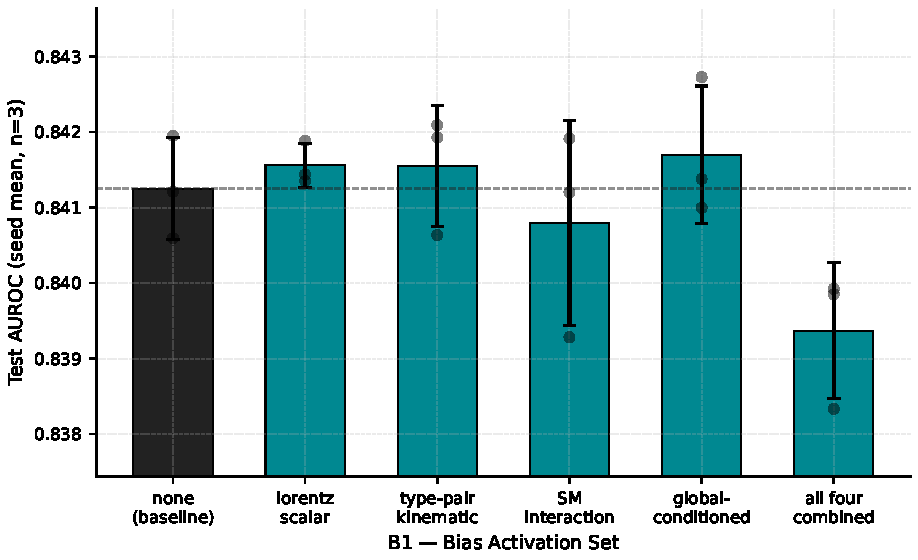
\includegraphics[width=\textwidth]{figures/ch5/figure-auroc_bar_by_bias_family}
\caption{Exp.\ 5A seed-mean test AUROC for all six \wandbaxis{B1}
configurations, with per-seed spread. Dashed line marks the \texttt{none}
baseline mean.}
\label{fig:5a_auroc_bar}
\end{figure}

Three observations follow directly from these results. First, no single
bias family moves the seed-mean AUROC by more than approximately one
inter-seed standard deviation away from the \texttt{none} baseline.
The three families that nominally improve accuracy (\texttt{lorentz\_scalar},
\texttt{typepair\_kinematic}, \texttt{global\_conditioned}) each gain at
most $+0.00045$ AUROC, which is smaller than the per-cell seed standard
deviation of the baseline itself. Second, \texttt{sm\_interaction} sits
$-0.00045$ below baseline, within one seed standard deviation. Third,
the full-combination cell is the only configuration whose mean (0.83937)
sits visibly below the baseline, at a deficit of approximately 0.002
AUROC. This result is consistent with mild optimisation interference when
multiple bias signals compete simultaneously for the same attention logit,
though it cannot be cleanly attributed to any single component without
further ablation.

The AUROC metric alone therefore does not reveal a meaningful benefit from
physics-informed attention biases at this model scale and seed budget. The
more informative question is whether the biases restructure attention
towards physically motivated patterns even when the classification boundary
shifts only modestly. The attention map analysis in
Section~\ref{sec:5a_attention_maps} addresses this.

\subsection{Attention structure: none versus full combination}
\label{sec:5a_attention_maps}

Attention weights are extracted at inference time by forwarding 2000
validation events through each model with the \texttt{capture\_attention}
flag enabled, then averaging over all heads, all layers, and all three
seeds. The physical token sub-block (18 particle tokens, positions 1--18
in the 21-token sequence; MET and MET-$\phi$ excluded) is projected onto a
$7\times 7$ type-pair grid by averaging attention from tokens of type $i$
to tokens of type $j$ for each ordered pair $(i, j)$ across events. The
seven physical types are: jet (1), b-jet (2), $e^+$ (3), $e^-$ (4),
$\mu^+$ (5), $\mu^-$ (6), photon (7).

\begin{figure}[h]
\centering
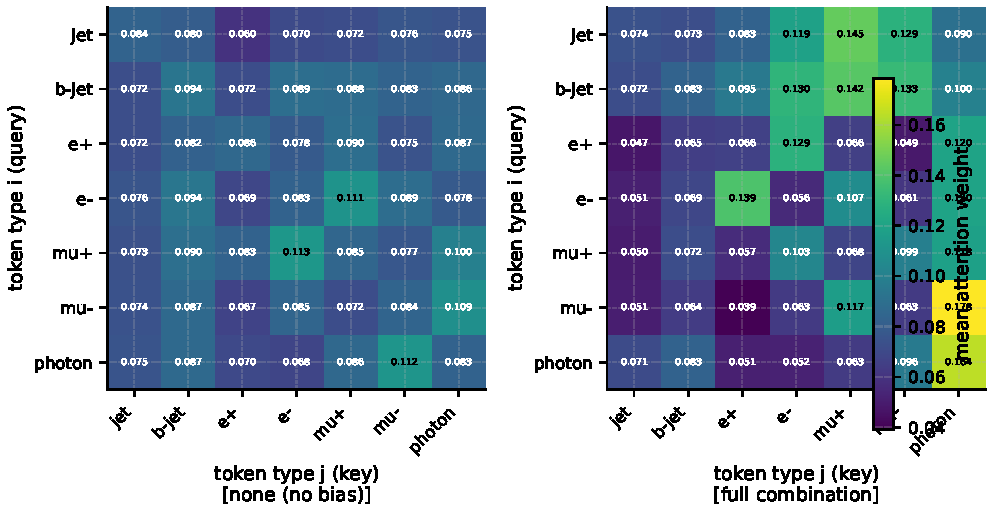
\includegraphics[width=\textwidth]{figures/ch5/figure-attn_typepair_mean_none_vs_full}
\caption{Type-pair mean attention weights for the \texttt{none} baseline
(left) and full-combination model (right), averaged over all heads, layers,
seeds, and 2000 validation events. Particle types: 1~=~jet, 2~=~b-jet,
3~=~$e^+$, 4~=~$e^-$, 5~=~$\mu^+$, 6~=~$\mu^-$, 7~=~photon. Pad tokens
excluded.}
\label{fig:5a_attn_mean}
\end{figure}

In the \texttt{none} baseline, type-pair attention weights occupy a
near-uniform range of 0.059--0.113. No pair dominates: the largest cell
($\mu^+ \to e^-$: 0.113) and the smallest (inferred from the stated range)
differ by only 0.054 units. The distribution is consistent with a model
that has learned to aggregate broad context without privileging specific
particle-type relationships.

The full-combination model produces a qualitatively different pattern.
Table~\ref{tab:5a_attn} lists the most strongly elevated and depressed
type-pair cells. The attention range widens to 0.039--0.178, a factor of
approximately $2.6$ relative to the baseline range of 0.054. Critically,
the elevated cells correspond to physically motivated interactions.

\begin{table}[h]
\centering\small
\begin{tabular}{llrl}
\toprule
Pair $(i \to j)$ & Mean attention & Physics interpretation \\
\midrule
$\mu^- \to \gamma$   & 0.178 & Lepton--photon (FSR / radiative return) \\
$\text{jet} \to \mu^+$  & 0.145 & Jet-embedded muon (semi-leptonic $b$-decay) \\
$\gamma \to \gamma$  & 0.164 & Photon self-attention (cluster isolation) \\
$b\text{-jet} \to \mu^+$ & 0.142 & Direct $b \to \mu$ semi-leptonic \\
$e^- \to e^+$        & 0.139 & Opposite-sign lepton pair ($Z$/$W$ decay) \\
$b\text{-jet} \to e^-$ & 0.130 & Semi-leptonic $b \to e$ \\
$e^+ \to e^-$        & 0.129 & Opposite-sign lepton pair \\
$\text{jet} \to \mu^-$ & 0.129 & Jet-embedded muon \\
$b\text{-jet} \to \mu^-$ & 0.133 & Semi-leptonic $b$-decay \\
\midrule
$\mu^- \to e^+$      & 0.039 & Same-charge mixed lepton (suppressed) \\
$e^+ \to \mu^-$      & 0.049 & Same-charge mixed lepton (suppressed) \\
\bottomrule
\end{tabular}
\caption{Selected type-pair mean attention weights under the full-combination
model (Exp.\ 5A), averaged over all heads, layers, seeds, and 2000
validation events. Pairs with mean attention $\geq 0.13$ are elevated;
pairs $\leq 0.05$ are depressed.}
\label{tab:5a_attn}
\end{table}

The pattern is interpretable in HEP terms. Lepton--photon pairs
($\mu^- \to \gamma$: 0.178) are associated with final-state radiation or
radiative $W/Z$ decays. Photon self-attention (0.164) reflects the
importance of photon isolation and cluster-shape information. The
$b$-jet-to-muon cells (0.142, 0.133) directly encode the semi-leptonic
$b$-decay topology relevant to top-quark reconstruction, where a $b$ quark
decays to a charm quark and a lepton. Opposite-sign lepton pairs
($e^- \to e^+$: 0.139, $e^+ \to e^-$: 0.129) are consistent with $Z$- or
$W$-boson leptonic decays in the multi-top system. By contrast, same-charge
mixed-lepton pairs ($\mu^- \to e^+$: 0.039) are strongly suppressed, as
expected for pairs that share no direct SM vertex in the $t\bar{t}t\bar{t}$
decay chain.

These results constitute the primary interpretability finding of the
chapter: the physics-informed biases do not substantially improve
classification accuracy on this dataset at this model scale, but they do
restructure the model's attention towards physically motivated particle-type
relationships. The model, when given structured priors through the bias
families, converges to an attention pattern that is broadly consistent with
HEP domain knowledge, even though the AUROC improvement is within seed
noise.

\begin{figure}[h]
\centering
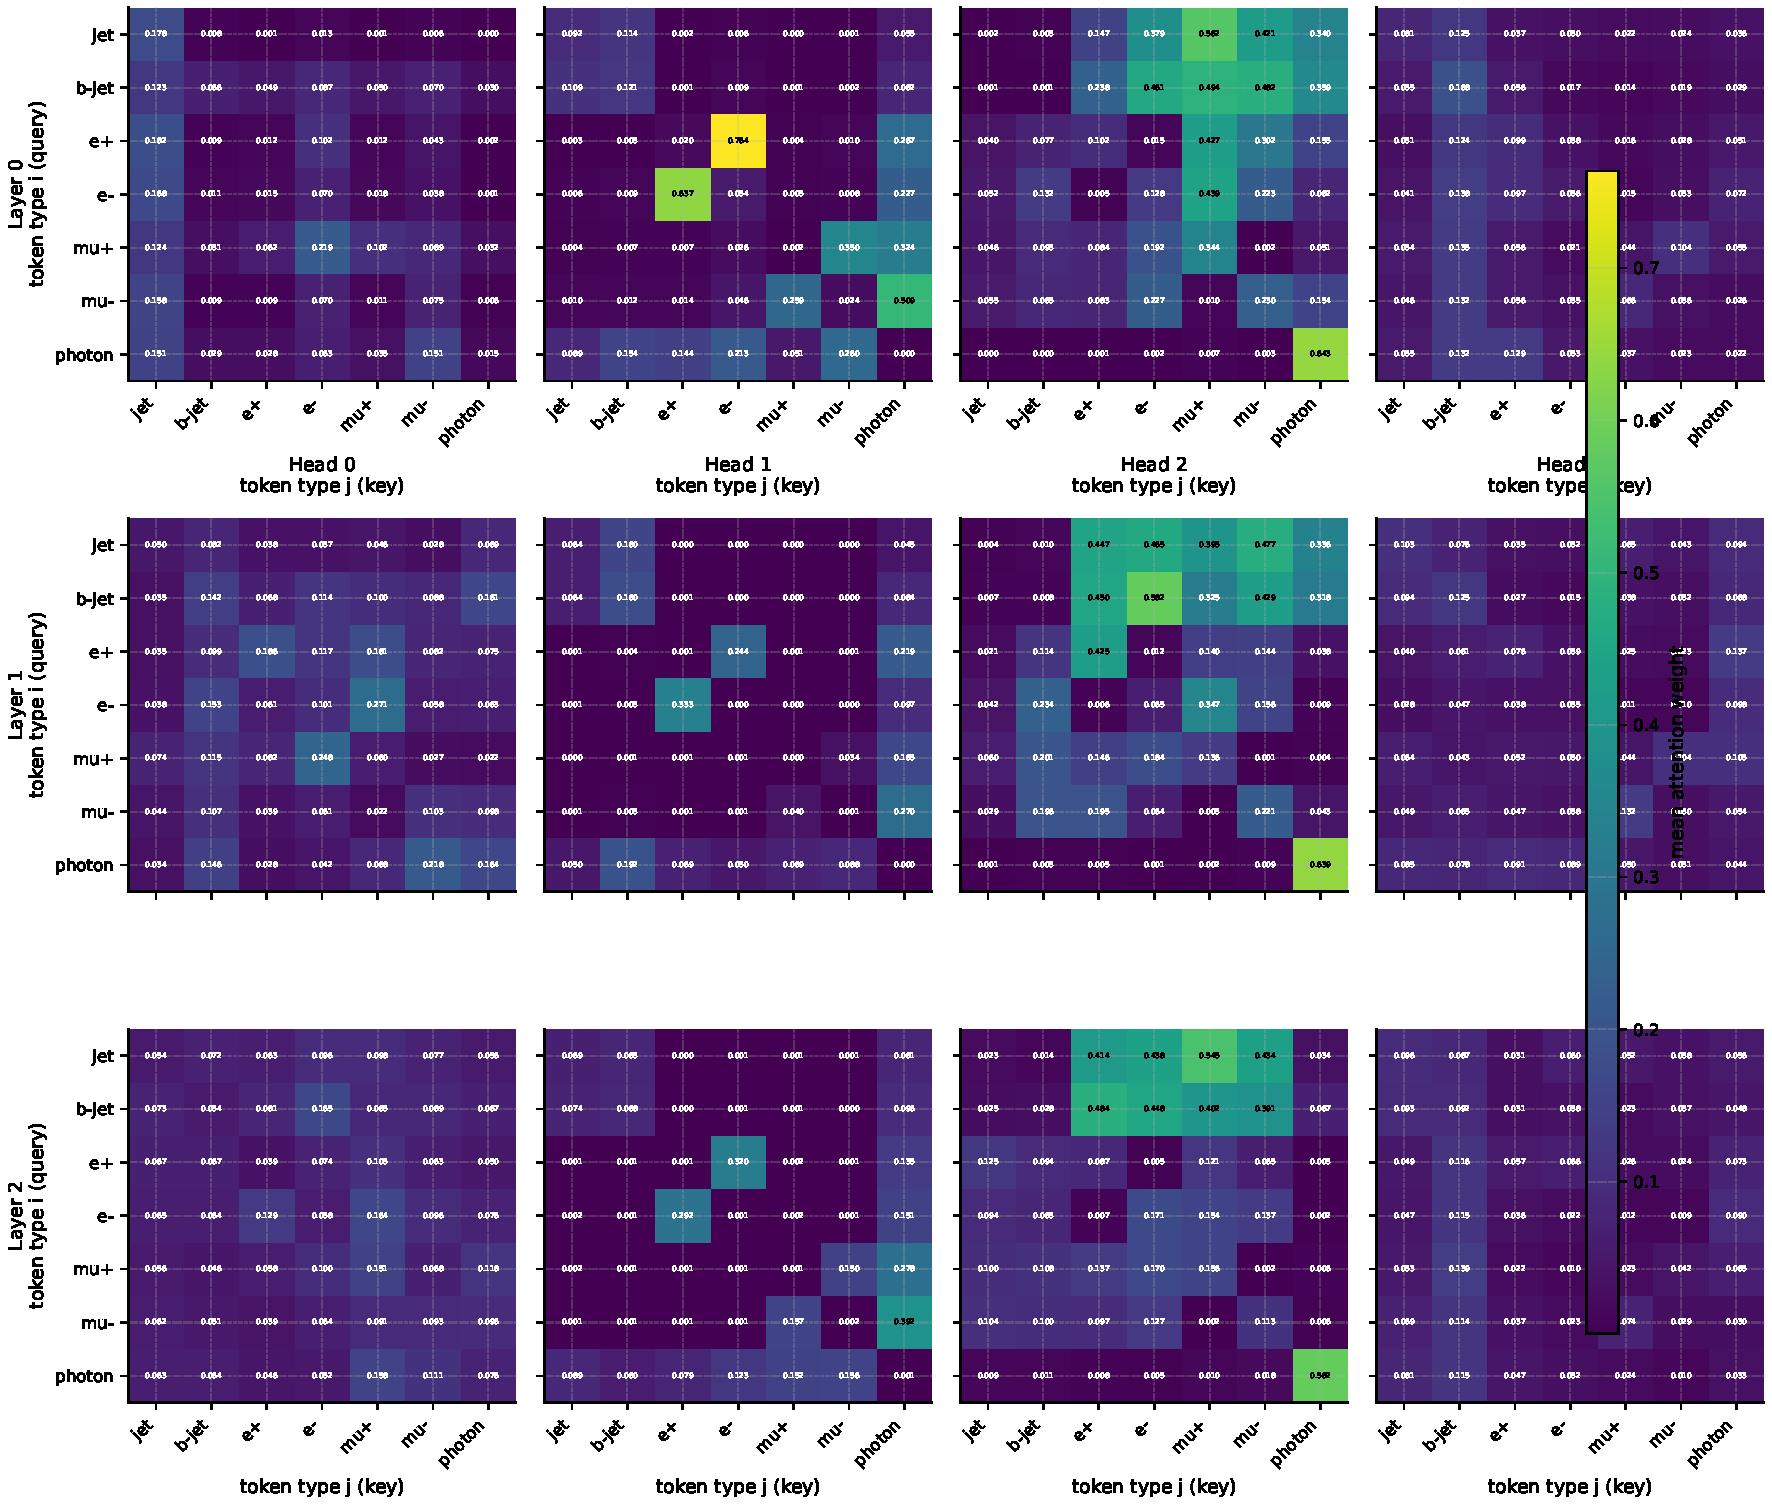
\includegraphics[width=\textwidth]{figures/ch5/figure-attn_typepair_per_head_full}
\caption{Type-pair attention weights for the full-combination model (seed 42),
shown separately for each of the 4 heads $\times$ 3 encoder layers.
Some heads specialise onto physically motivated pairs while others retain
near-uniform attention.}
\label{fig:5a_attn_per_head_full}
\end{figure}

The per-head, per-layer attention grids (available in the supplementary
figures) show that the structured pattern is not uniform across all twelve
head--layer combinations. Some heads retain near-uniform attention while
others specialise strongly onto physically motivated pairs, consistent with
the expectation that multi-head attention allows functional specialisation.


% ──────────────────────────────────────────────
\section{Lorentz feature set and bias network (Exp.\ 5B)}
\label{sec:5b}

\subsection{Experimental design}

The Lorentz-scalar bias sub-network (\wandbaxis{B1-L}) computes a pairwise
attention score from Lorentz-invariant quantities derived from pairs of
four-momenta. Experiment 5B asks three questions about the internal design
of this sub-network: which kinematic features are most informative
(\wandbaxis{B1-L1}), whether replacing the standard pointwise MLP with a
Kolmogorov--Arnold Network (KAN) improves the learned response
(\wandbaxis{B1-L2}), and whether a per-feature sparse gate (\wandbaxis{B1-L5})
can learn to prune uninformative features automatically. Sixty runs span
five feature sets, two MLP types, and two gating settings, at three seeds
each.

\begin{table}[h]
\centering\small
\begin{tabular}{llr}
\toprule
Axis & Values & Levels \\
\midrule
\wandbaxis{B1-L1} — Feature set & \texttt{[deltaR]}                                      & 5 \\
 & \texttt{[m2]}                                         & \\
 & \texttt{[m2, deltaR]}                                 & \\
 & \texttt{[log\_kt, z, deltaR, log\_m2]}               & \\
 & \texttt{[m2, deltaR, log\_m2, log\_kt, z, deltaR\_ptw]} & \\
\wandbaxis{B1-L2} — MLP type    & \texttt{standard}, \texttt{kan}                     & 2 \\
\wandbaxis{B1-L5} — Sparse gating & \texttt{false}, \texttt{true}                     & 2 \\
Seeds (\wandbaxis{R5})           & 42, 123, 314                                          & 3 \\
\midrule
Total & & \textbf{60} \\
\bottomrule
\end{tabular}
\caption{Exp.\ 5B design. B1~=~\texttt{lorentz\_scalar} throughout.
B1-L3 (hidden dim) and B1-L4 (per-head mode) are held at defaults.}
\label{tab:5b_design}
\end{table}

All kinematic features are computed from z-score-normalised four-vectors.
An important consequence of this normalisation is that the pairwise
invariant mass $m^2$ collapses near zero on the normalised scale (validation
median of $m^2$ is $0.000$; 95th percentile is $2.47$). The logarithmic
variant $\log m^2$ collapses further (validation median
$\approx \log(10^{-6}) \approx -13.8$). This means that any claim about
``learning the $W$-boson or top-quark mass peak'' is not supported by these
checkpoints; such an analysis would require either removing input
normalisation or de-normalising the feature axis. By contrast, $\Delta R$,
$\log k_T$, and $z$ remain well-behaved on the normalised scale ($\Delta R$
at the 5th and 95th percentiles: $0.79$ and $4.17$ respectively), and
interpretability arguments based on those features are on firmer ground.

\subsection{AUROC results}

Table~\ref{tab:5b_auroc} reports seed-mean AUROC for all 20 (feature set,
MLP type, gating) cells. The full bar chart is shown as Figure~\ref{fig:5b_auroc_bar}.

\begin{figure}[h]
\centering
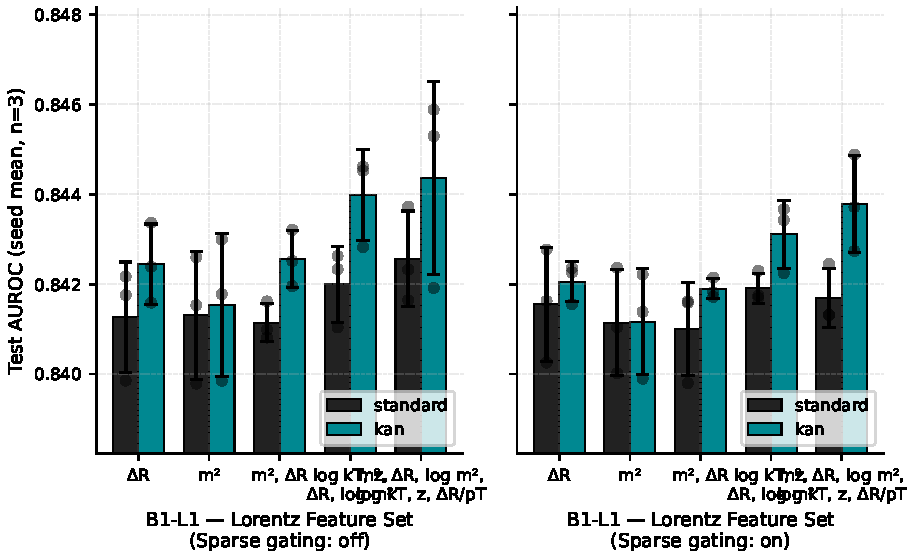
\includegraphics[width=\textwidth]{figures/ch5/figure-auroc_bar_by_lorentz}
\caption{Exp.\ 5B seed-mean test AUROC for all 20 (feature set, MLP type,
gating) cells, with per-seed spread. KAN consistently meets or exceeds the
standard MLP; richer feature sets produce higher AUROC; sparse gating
provides no benefit.}
\label{fig:5b_auroc_bar}
\end{figure}

\begin{table}[h]
\centering\small
\begin{tabular}{llllrr}
\toprule
Feature set & MLP type & Gating & Mean AUROC & Seed std \\
\midrule
$\Delta R$                                & standard & off & 0.84126 & 0.00123 \\
$\Delta R$                                & kan      & off & 0.84245 & 0.00089 \\
$\Delta R$                                & standard & on  & 0.84155 & 0.00126 \\
$\Delta R$                                & kan      & on  & 0.84206 & 0.00044 \\
\addlinespace
$m^2$                                     & standard & off & 0.84131 & 0.00142 \\
$m^2$                                     & kan      & off & 0.84154 & 0.00159 \\
$m^2$                                     & standard & on  & 0.84114 & 0.00118 \\
$m^2$                                     & kan      & on  & 0.84117 & 0.00118 \\
\addlinespace
$m^2$, $\Delta R$                          & standard & off & 0.84114 & 0.00042 \\
$m^2$, $\Delta R$                          & kan      & off & 0.84256 & 0.00063 \\
$m^2$, $\Delta R$                          & standard & on  & 0.84100 & 0.00104 \\
$m^2$, $\Delta R$                          & kan      & on  & 0.84190 & 0.00022 \\
\addlinespace
$\log k_T$, $z$, $\Delta R$, $\log m^2$   & standard & off & 0.84200 & 0.00085 \\
$\log k_T$, $z$, $\Delta R$, $\log m^2$   & kan      & off & 0.84399 & 0.00101 \\
$\log k_T$, $z$, $\Delta R$, $\log m^2$   & standard & on  & 0.84191 & 0.00034 \\
$\log k_T$, $z$, $\Delta R$, $\log m^2$   & kan      & on  & 0.84311 & 0.00076 \\
\addlinespace
$m^2$, $\Delta R$, $\log m^2$, $\log k_T$, $z$, $\Delta R/p_T$  & standard & off & 0.84257 & 0.00106 \\
$m^2$, $\Delta R$, $\log m^2$, $\log k_T$, $z$, $\Delta R/p_T$  & kan      & off & \textbf{0.84436} & 0.00214 \\
$m^2$, $\Delta R$, $\log m^2$, $\log k_T$, $z$, $\Delta R/p_T$  & standard & on  & 0.84170 & 0.00065 \\
$m^2$, $\Delta R$, $\log m^2$, $\log k_T$, $z$, $\Delta R/p_T$  & kan      & on  & 0.84378 & 0.00107 \\
\bottomrule
\end{tabular}
\caption{Exp.\ 5B seed-mean test AUROC ($n = 3$ per cell). The
\texttt{none} baseline from Exp.\ 5A is $0.84125 \pm 0.00068$.
Best cell highlighted. Gating ``on'' = \wandbaxis{B1-L5}~=~\texttt{true}.}
\label{tab:5b_auroc}
\end{table}

Three consistent trends emerge from the table. First, within every
(feature-set, gating) pairing, the \texttt{kan} MLP equals or exceeds the
\texttt{standard} MLP in seed-mean AUROC. The largest gap appears in the
six-feature, gating-off configuration ($+0.0018$ AUROC), which equals
approximately one seed standard deviation. The global best cell (6-feature,
KAN, gate off: $0.84436$) sits roughly $+0.0031$ above the Exp.\ 5A
\texttt{none} baseline ($0.84125$), a margin comparable to several per-cell
seed standard deviations. Second, richer Lorentz feature panels
systematically produce higher AUROC than single-feature panels, particularly
when paired with the KAN. The four- and six-feature sets consistently
outperform the $\Delta R$-only and $m^2$-only single-feature sets; this
trend is visible in both the standard and KAN columns. Third, sparse gating
provides no benefit at this scale and seed budget: gate-on cells tend to
sit slightly below their gate-off counterparts in the same (feature, MLP)
row, by approximately $0.0005$--$0.0009$ AUROC.

\subsection{KAN spline structure and gate values}
\label{sec:5b_interp}

The expressive difference between KAN and standard MLP is visible not only
in AUROC but in the learned attention-bias functions themselves. In the
single-feature ($\Delta R$) configuration with gating off, the seed-mean
bias function spans a range of $0.99$ arbitrary units under the KAN, versus
$0.46$ under the standard MLP: a factor of approximately two. In the
partial-dependence view of the four-feature configuration (other features
held at validation medians), the standard MLP learns almost no log-$k_T$
dependence (range $\approx 0.05$), while the KAN learns a structured curve
with range $\approx 0.65$. This result is consistent with the KAN's
capacity to model sharp univariate edges with a small parameter budget
through its B-spline basis. The KAN therefore extracts more functional
structure from the pairwise kinematic features, which is reflected in the
consistent AUROC advantage.

\begin{figure}[h]
\centering
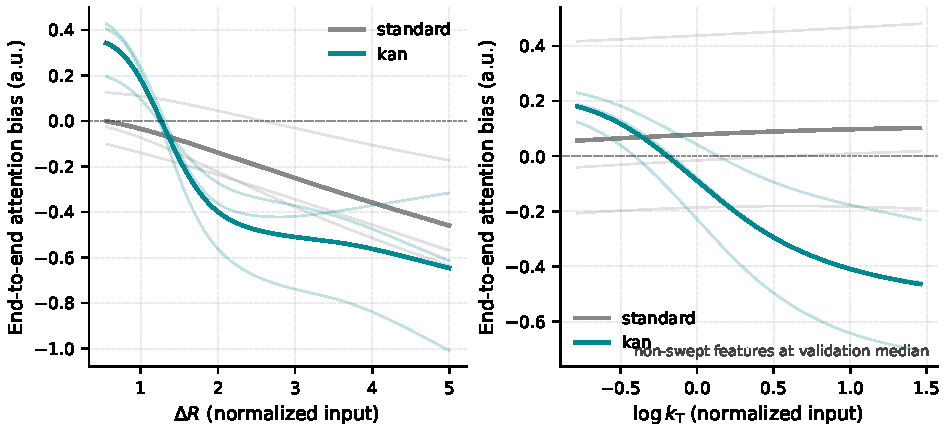
\includegraphics[width=0.7\textwidth]{figures/ch5/figure-1d_bias_kan_vs_standard}
\caption{Learned 1D bias function for the $\Delta R$-only feature set
comparing KAN (blue) and standard MLP (orange), averaged over three seeds.
The KAN spans a range of $\approx 0.99$ attention units versus $\approx 0.46$
for the standard MLP.}
\label{fig:5b_bias_1d}
\end{figure}

The per-module gate, $\tanh(g)$, converged to a positive value in every one
of the 60 Exp.\ 5B runs, confirming that the Lorentz bias is non-trivially
active throughout the cohort. KAN modules average $\tanh(g) \approx 0.28
\pm 0.08$ versus $0.22 \pm 0.10$ for standard modules. The higher gate for
KAN runs echoes the AUROC finding: the network allows more of the KAN's
richer signal through its multiplicative gate.

Despite the gate being consistently open, the sparse feature-gating
mechanism (\wandbaxis{B1-L5}) does not learn meaningful per-feature
selection. The sigmoid gate values $\sigma(\text{feature\_gates})$ remain
within $0.49$--$0.62$ across all 15 sparse-on KAN runs, barely departing
from their initialisation at $\sigma(0) = 0.5$.  The only feature whose
mean gate drifts slightly below $0.5$ is $\log m^2$, which is precisely
the feature whose input distribution collapses near $-13.8$ under z-score
normalisation. Even this drift is modest ($\approx 0.494 \pm 0.022$),
and no feature is pruned in any run. The effect on AUROC is therefore a
slight attenuation of every feature's amplitude simultaneously, with no
compensating benefit from pruning, which explains the small but systematic
gap between gate-on and gate-off cells.

\begin{figure}[h]
\centering
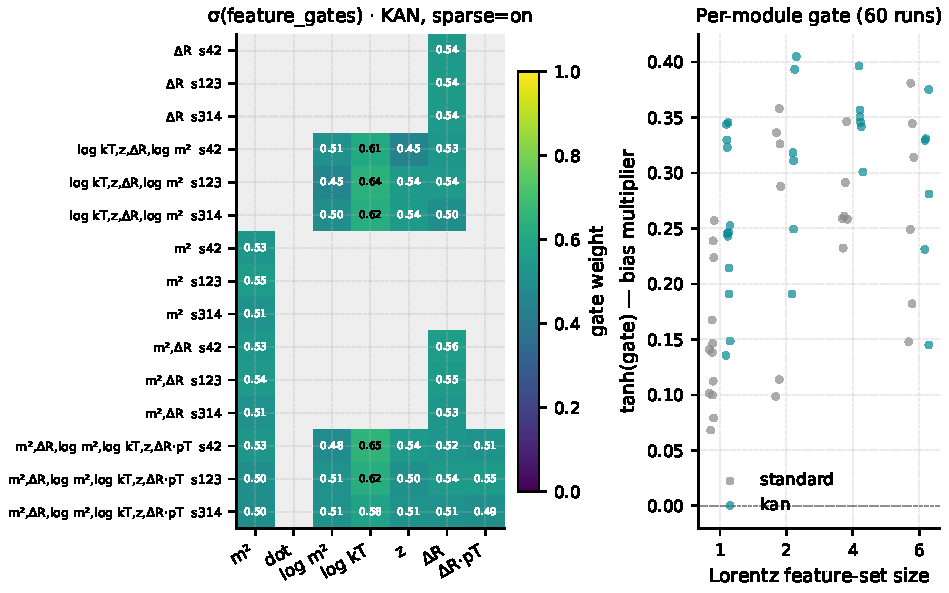
\includegraphics[width=\textwidth]{figures/ch5/figure-feature_gates_and_module_gate}
\caption{Left: per-feature sparse gate values $\sigma(\text{gate})$ for all
Exp.\ 5B sparse-on KAN runs; all gates remain within $0.49$--$0.62$,
indicating no meaningful feature pruning. Right: module-level scalar gate
$\tanh(g)$ for KAN (blue) and standard (orange) MLP runs across the full
cohort.}
\label{fig:5b_gates}
\end{figure}

One caveat for the spline-shape analysis is that the KAN B-spline grid is
fixed at its initialisation throughout training: \texttt{update\_grid} is
not called during the forward pass, which was confirmed by state-dict
inspection of the \texttt{mlp.0.grid} key in the saved checkpoints. The
spline expressivity is therefore bounded by the initial grid resolution
and not by adaptive grid relocation. More adaptive grid training could in
principle widen the gap further.


% ──────────────────────────────────────────────
\section{Type-pair initialisation and freeze (Exp.\ 5C)}
\label{sec:5c}

\subsection{Experimental design}

The type-pair kinematic bias (\wandbaxis{B1-T}) maintains a learnable
$N_\mathrm{type}\times N_\mathrm{type}$ table of attention score offsets,
one per ordered particle-type pair. Experiment 5C varies two design choices:
the initialisation strategy (\wandbaxis{B1-T1}) and whether the table is
frozen after initialisation (\wandbaxis{B1-T2}). Three initialisation
modes are tested: \texttt{none} (zero start, free to train), \texttt{binary}
(a $\{0, -5\}$ mask encoding which SM vertices are allowed or forbidden),
and \texttt{fixed\_coupling} (the physics-motivated initialisation, with
magnitudes proportional to SM coupling constants). A frozen table
(\texttt{freeze\_table~=~true}) acts as a fixed physics prior; a free
table is adjusted by gradient descent from its initialised state. Fifteen
runs cover five cells (the \texttt{none}--frozen combination is excluded,
as there is no table to freeze) at three seeds each.

\begin{table}[h]
\centering\small
\begin{tabular}{llr}
\toprule
Axis & Values & Levels \\
\midrule
\wandbaxis{B1-T1} — Init & \texttt{none}, \texttt{binary}, \texttt{fixed\_coupling} & 3 \\
\wandbaxis{B1-T2} — Freeze & \texttt{false}, \texttt{true} (only when init $\neq$ \texttt{none}) & — \\
Seeds (\wandbaxis{R5})     & 42, 123, 314 & 3 \\
\midrule
Total & & \textbf{15} \\
\bottomrule
\end{tabular}
\caption{Exp.\ 5C design. B1~=~\texttt{typepair\_kinematic} throughout.
B1-T3 (kinematic gate), B1-T4 (kinematic feature), and B1-T5 (mask value)
are held at defaults.}
\label{tab:5c_design}
\end{table}

\subsection{Performance results}

Table~\ref{tab:5c_auroc} reports seed-mean AUROC for the five cells.
The local \texttt{none}-init baseline here (0.84205) is slightly above the
Exp.\ 5A \texttt{none} cell (0.84125), a difference attributable to the
different sweep configuration and cohort, not to a change in the architecture.

\begin{table}[h]
\centering\small
\begin{tabular}{lllrrl}
\toprule
Init & Freeze & Mean AUROC & Seed std & $\Delta$ vs \texttt{none} \\
\midrule
\texttt{none}           & free   & 0.84205 & 0.00081 & --- \\
\texttt{binary}         & free   & 0.84075 & 0.00046 & $-0.00130$ \\
\texttt{binary}         & frozen & 0.84131 & 0.00065 & $-0.00074$ \\
\texttt{fixed\_coupling}& free   & 0.84175 & 0.00102 & $-0.00030$ \\
\texttt{fixed\_coupling}& frozen & 0.84138 & 0.00046 & $-0.00067$ \\
\bottomrule
\end{tabular}
\caption{Exp.\ 5C seed-mean test AUROC ($n = 3$ per cell). All four
physics-initialised cells sit below the \texttt{none} baseline within one
to two seed standard deviations.}
\label{tab:5c_auroc}
\end{table}

All four physics-initialised cells sit below the \texttt{none} baseline in
seed mean, by margins of $0.0003$--$0.0013$ AUROC. These deltas are within
one to two per-cell seed standard deviations and should not be interpreted
as a meaningful performance deficit. The \texttt{fixed\_coupling}
initialisation consistently outperforms \texttt{binary} by approximately
$0.0006$--$0.0010$ AUROC regardless of freeze state, but again at the noise
floor. Freezing the table has small, non-monotonic effects: it slightly
improves \texttt{binary} ($+0.00056$) and slightly reduces
\texttt{fixed\_coupling} ($-0.00037$), both within seed variance.

The AUROC results therefore suggest neither a benefit from SM-seeded
initialisation nor a cost from freezing the physics prior, at this seed
budget and model scale.

\subsection{Learned table structure}

The more informative view comes from inspecting the converged type-pair
tables directly. The state-dict key
\texttt{bias\_composer.bias\_modules.\allowbreak{}typepair\_kinematic.\allowbreak{}table\_raw}
has shape $[8,8]$; the symmetric form is reconstructed as
$\frac{1}{2}(T + T^\top)$ and the padding row and column are removed,
leaving a $7\times 7$ active matrix. Table~\ref{tab:5c_table_stats}
summarises key scalar statistics.

\begin{table}[h]
\centering\small
\begin{tabular}{llrlrl}
\toprule
Init & Freeze & Gate ($\tanh g$, mean $\pm$ std) & Frobenius norm & Drift from init \\
\midrule
\texttt{none}            & free   & $0.234 \pm 0.015$ & 0.434  & 0.944 (= norm) \\
\texttt{binary}          & free   & $0.097 \pm 0.012$ & 27.044 & 0.868 \\
\texttt{binary}          & frozen & $0.094 \pm 0.013$ & 27.295 & 0.000 (frozen) \\
\texttt{fixed\_coupling} & free   & $0.104 \pm 0.015$ & 26.848 & 0.930 \\
\texttt{fixed\_coupling} & frozen & $0.101 \pm 0.015$ & 27.094 & $\approx 0$ \\
\bottomrule
\end{tabular}
\caption{Exp.\ 5C per-group learned-table statistics. Gate = $\tanh(g)$
averaged over 3 seeds. Frobenius norm computed on the $7\times 7$ active
sub-matrix. Drift from init = Frobenius distance between the converged
seed-mean table and the reference initialisation.}
\label{tab:5c_table_stats}
\end{table}

The \texttt{none}-init table starts from zero and converges to a
small-magnitude matrix (Frobenius $0.43$), with values scattered in
$[-0.16, +0.12]$ showing no discernible SM-interaction pattern at $n=3$
seeds. Its gate is notably higher ($0.234$) than any physics-initialised
group ($0.094$--$0.104$), consistent with the network opening the gate
further when the table provides a weak prior and all type pairs look equally
neutral at initialisation.

The \texttt{fixed\_coupling}-free table preserves the SM structure through
training. QCD quark--quark pairs (jet--jet: $+1.22$, jet--b-jet: $+1.17$,
b-jet--b-jet: $+1.23$) retain large positive values; EW lepton pairs
($e^+e^-$: $+0.54$, $\mu^+\mu^-$: $+0.89$) retain intermediate positive
values; and all non-interacting pairs remain near the mask value of $-5.0$.
The Frobenius drift from initialisation is $0.930$, indicating that
training adjusts the coupling-constant magnitudes by roughly $\pm 0.1$--$0.3$
rather than restructuring the topology. This is a notable result: the
network broadly respects the SM interaction hierarchy encoded at
initialisation, even when the gradient is free to reorganise the table
entirely.

\begin{figure}[h]
\centering
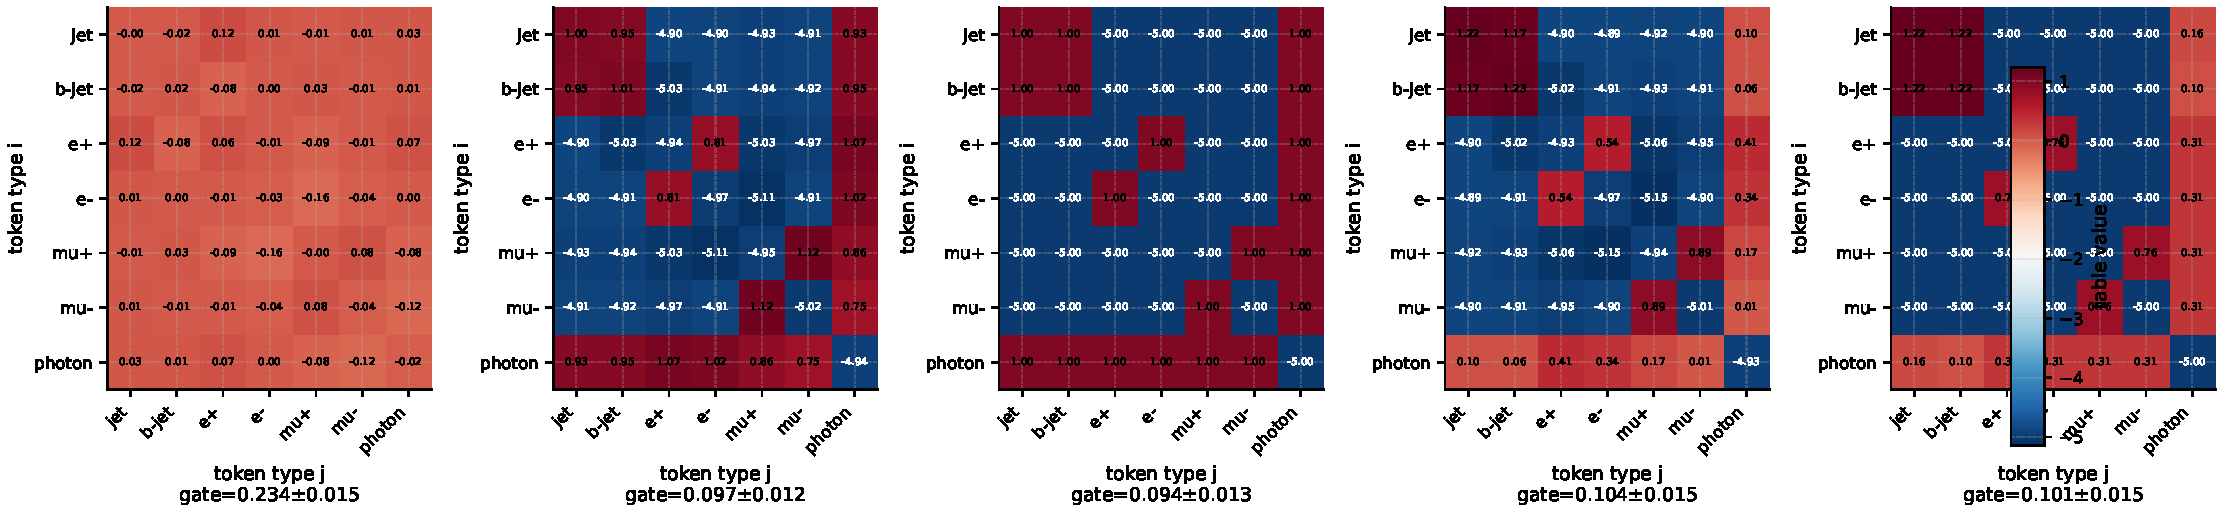
\includegraphics[width=\textwidth]{figures/ch5/figure-typepair_learned_tables}
\caption{Converged type-pair tables ($7\times 7$ active sub-matrix) for all
five Exp.\ 5C groups, averaged over three seeds. The
\texttt{fixed\_coupling}-free table preserves the SM coupling hierarchy;
the \texttt{none}-init table remains near-uniform.}
\label{fig:5c_tables}
\end{figure}

\begin{figure}[h]
\centering
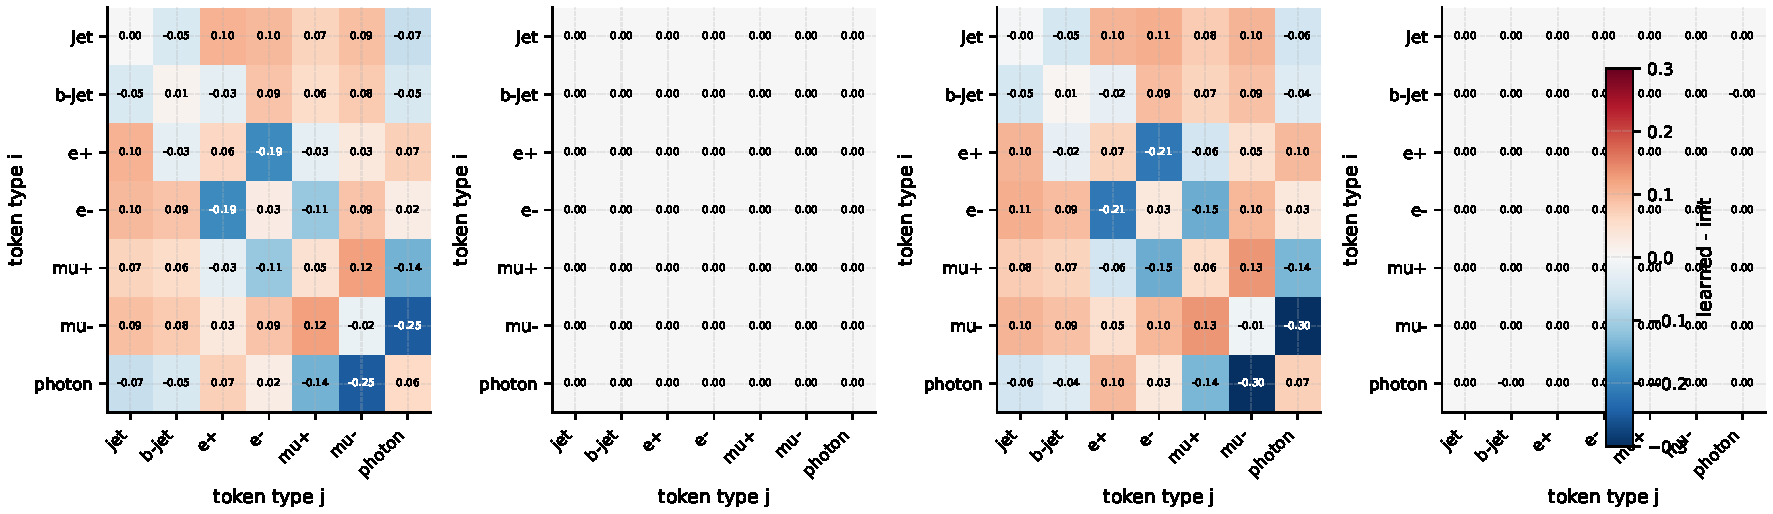
\includegraphics[width=\textwidth]{figures/ch5/figure-typepair_diff_from_init}
\caption{Per-cell table drift from initialisation for the free-table groups.
\texttt{fixed\_coupling}-free (top) shows small, structured adjustments
($\pm 0.1$--$0.3$) with the SM topology intact;
\texttt{binary}-free (bottom) shows larger drift at active entries.}
\label{fig:5c_diff}
\end{figure}

The \texttt{binary}-free group shows an analogous pattern (same mask
positions preserved) but with higher drift (0.868 vs 0.930), reflecting the
fact that the binary initialisation provides structural topology but no
coupling-constant scale, leaving active entries more exposed to gradient
learning. The frozen groups confirm the mechanism functions correctly
(freeze drift $\approx 6.6 \times 10^{-8}$ for \texttt{fixed\_coupling}-frozen).

Taken together, the results suggest that the SM \texttt{fixed\_coupling}
initialisation provides a structural prior that training broadly preserves,
but that its effective attention contribution, modulated by the scalar gate
($\tanh(g) \approx 0.10$), is too small to produce a measurable AUROC
improvement at this configuration. The \texttt{none}-init group, starting
from a flat table, fails to recover a physics-consistent structure at three
seeds --- the table remains near-uniform, indicating that the inductive bias
from the initialisation is important for guiding the table to a structured
solution.


% ──────────────────────────────────────────────
\section{SM interaction mode (Exp.\ 5D)}
\label{sec:5d}

Experiment 5D tests whether increasing physical fidelity in the SM
interaction prior produces measurable gains. The \texttt{sm\_interaction}
bias family encodes SM topology as a fixed or modulated additive bias on
attention logits; axis \wandbaxis{B1-S1} selects among three modes:
\texttt{binary} (a $\{0, -5\}$ allowed/forbidden mask), \texttt{fixed\_coupling}
(coupling constants at a fixed energy scale), and
\texttt{running\_coupling} ($\alpha_s(Q^2)$ evaluated at the pairwise
momentum transfer). Nine runs cover all three modes at three seeds each.

\begin{table}[h]
\centering\small
\begin{tabular}{llr}
\toprule
Axis & Values & Levels \\
\midrule
\wandbaxis{B1-S1} — SM mode & \texttt{binary}, \texttt{fixed\_coupling}, \texttt{running\_coupling} & 3 \\
Seeds (\wandbaxis{R5})       & 42, 123, 314 & 3 \\
\midrule
Total & & \textbf{9} \\
\bottomrule
\end{tabular}
\caption{Exp.\ 5D design. B1~=~\texttt{sm\_interaction} throughout.
B1-S2 (mask value) held at default.}
\label{tab:5d_design}
\end{table}

Table~\ref{tab:5d_auroc} reports seed-mean AUROC. The reference \texttt{none}
baseline from Exp.\ 5A ($0.84125 \pm 0.00068$) is used for comparison, as
Exp.\ 5D does not include an explicit \texttt{none} cell; both cohorts
share the same encoder hyperparameters and seed list, so the cross-cohort
comparison is reasonable.

\begin{table}[h]
\centering\small
\begin{tabular}{lrrl}
\toprule
B1-S1 mode & Mean AUROC & Seed std & $\Delta$ vs 5A \texttt{none} \\
\midrule
\texttt{binary}           & 0.84140 & 0.00050 & $+0.00015$ \\
\texttt{fixed\_coupling}  & 0.84146 & 0.00091 & $+0.00021$ \\
\texttt{running\_coupling}& 0.84108 & 0.00081 & $-0.00018$ \\
\bottomrule
\end{tabular}
\caption{Exp.\ 5D seed-mean test AUROC ($n = 3$ per cell). All three modes
are within $\pm 0.0002$ AUROC of the Exp.\ 5A \texttt{none} baseline.}
\label{tab:5d_auroc}
\end{table}

All three SM-interaction modes sit within $\pm 0.0002$ AUROC of the
\texttt{none} baseline, and the three modes span only $\approx 0.0004$
AUROC among themselves. Both magnitudes are at or below the per-cell seed
standard deviation, making no mode distinguishable from another within this
seed budget. The nominal ranking (\texttt{fixed\_coupling} $>$
\texttt{binary} $>$ \texttt{running\_coupling}) is consistent with the
\texttt{running\_coupling} mode being the most parameter-rich and therefore
most exposed to optimisation noise at fixed hyperparameters, but this
interpretation should not be treated as a directional finding at $n=3$ seeds.

\begin{figure}[h]
\centering
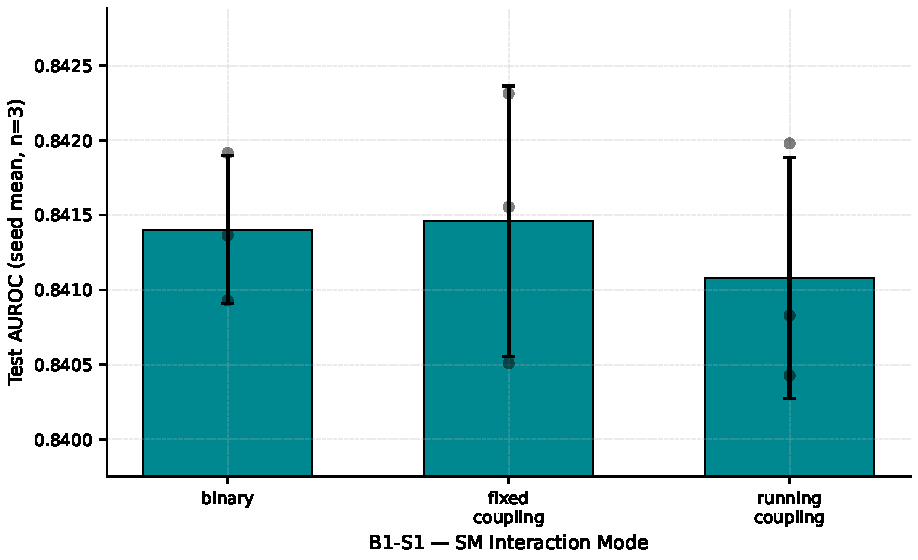
\includegraphics[width=0.7\textwidth]{figures/ch5/figure-auroc_bar_by_sm_mode}
\caption{Exp.\ 5D seed-mean test AUROC for the three \wandbaxis{B1-S1}
modes, with per-seed spread. Dashed line marks the Exp.\ 5A
\texttt{none} baseline. All three modes are within $\pm 0.0002$ AUROC of
the baseline.}
\label{fig:5d_auroc_bar}
\end{figure}

The SM interaction prior as implemented in Exp.\ 5D is therefore a null
result on the AUROC axis at this model scale. Whether the prior is active
in the attention pattern is a question for a future attention-map follow-up
analogous to the Exp.\ 5A analysis (currently staged but not yet run).
For the purpose of the downstream best-model selection in Ch.\,8, the
\texttt{fixed\_coupling} mode is carried forward as the default SM setting
on the grounds of physical motivation, accepting that the performance
difference is negligible.


% ──────────────────────────────────────────────
\section{Chapter synthesis}
\label{sec:5_synthesis}

This chapter set out to ask whether physics-informed attention biases
improve 4-tops-versus-background classification, and what those biases
reveal about the model's internal organisation of particle relationships.
The AUROC results across all four sub-experiments are consistent and
unambiguous: no single bias family, and no configuration within any
family, produces a performance gain that is clearly separable from seed
variance at $n=3$ seeds per cell. The total AUROC range across all 102
runs is approximately $0.838$--$0.846$, with per-cell seed standard
deviations of order $0.001$. The full-combination configuration in Exp.\ 5A
is the only cell that sits visibly below the \texttt{none} baseline
($\approx -0.002$ AUROC), suggestive of optimisation interference from
multiple simultaneous bias signals.

The interpretability results tell a richer story. When all four bias
families are active, the model sharpens type-pair attention onto
physically motivated particle relationships: the attention range widens by
a factor of $2.6$ (from $0.054$ in the \texttt{none} baseline to $0.139$
in the full-combination model), and the most elevated pairs are lepton--photon
($\mu^- \to \gamma$: $0.178$), photon self-attention ($0.164$), b-jet-to-muon
pairs consistent with semi-leptonic $b$-decay ($0.142$, $0.133$), and
opposite-sign lepton pairs consistent with $Z/W$ decay ($e^- \to e^+$:
$0.139$). Same-charge mixed-lepton pairs, which lack a common SM vertex,
are strongly suppressed. These patterns demonstrate that physics-informed
biases restructure the model's attention rather than merely adding capacity.

Within the Lorentz-scalar family, KAN sub-networks consistently learn
richer bias functions than standard MLPs across the same feature sets,
with the largest gap at the six-feature configuration ($+0.0018$ AUROC,
bias-function range $2\times$ wider). Sparse feature gating, however,
converges to the all-open state ($\sigma \approx 0.5$) in every run,
providing no automatic feature selection at this training budget.

The type-pair table analysis shows that the SM \texttt{fixed\_coupling}
initialisation provides a structural prior that training broadly respects:
QCD quark--quark and EW lepton-pair entries retain their physics-consistent
magnitudes through gradient descent, with Frobenius drift $0.930$ from the
initialisation. By contrast, a zero-start (\texttt{none}-init) table fails
to recover a physics-consistent structure at $n=3$ seeds, suggesting that
the inductive bias from a physics-motivated initialisation is beneficial
for interpretability even when it does not shift accuracy.

The practical takeaway for the remainder of the thesis is that
physics-informed attention biases do not change the operating point of the
classifier at the model scale studied in this chapter. Their value is
interpretive: they make the model's attention patterns legible in HEP
terms. For downstream experiments in Ch.\,6 and Ch.\,8, the chapter
baseline carries forward the \texttt{lorentz\_scalar} bias in the
six-feature, standard-MLP, gating-off configuration as the default B1
setting, on the grounds that it provides the most consistent, modest AUROC
benefit without the optimisation risk of the full-combination stack.

\begin{table}[h]
\centering\small
\begin{tabular}{llr}
\toprule
Experiment & Primary axes & Runs \\
\midrule
5A — Family comparison    & \wandbaxis{B1}                            & 18 \\
5B — Lorentz ablation     & \wandbaxis{B1-L1}, \wandbaxis{B1-L2}, \wandbaxis{B1-L5} & 60 \\
5C — Type-pair table      & \wandbaxis{B1-T1}, \wandbaxis{B1-T2}      & 15 \\
5D — SM interaction mode  & \wandbaxis{B1-S1}                         &  9 \\
\midrule
\textbf{Total} & & \textbf{102} \\
\bottomrule
\end{tabular}
\caption{Chapter 5 run summary.}
\label{tab:ch5_summary}
\end{table}
